% !TEX root = _yoko.tex

% ==========================================
% プロジェクト予稿（1P）の本文
% ==========================================

\section{はじめに}
音楽は，今日多くの人にとって日常の一部となっており，その楽しみ方も多岐にわたる．音楽は人々の感情や想いを表現し共有する手段の１つとなっている．本研究では，作品制作を通して空間における音楽映像体験を提供することを目的とする．
%作品制作では，を誰もが再現できるような簡易的な素材と技術を用いて楽器の生演奏に合わせた空間演出を行う． 

\section{演出表現における音楽要素}
音楽は様々な要素から成り立っており，演出表現を行う際に大きな役割を持つ．

演出表現に関わる音楽の要素には，大きく「譜面的要素」と「背景的要素」が挙げられる．
譜面的要素とは，音高や音量の変化，コード進行による曲調の変化，楽器構成などである．
聴衆にとって感情や認知などに影響をもたらすことが多く，歌詞や曲調を手掛かりとした照明演出において取り入れられてる\cite{Kanno22}．
一方，背景的要素は，曲の制作過程や，演奏者の想い，何かの主題歌であるかどうかなどの情報などである．
聴衆に具体的な情景を想起させるための手掛かりとなることが多い．
これらの要素を踏まえ，福知山公立大学3201の教室を利用して，複数の作品制作を行った．

\section{作品の世界観を再現する演出表現}
1つ目の作品としてアラジンの主題歌である「A Whole New World」\cite{Aladdin}のピアノ演奏に合わせた演出表現を行った．この作品では自身が演奏者として演奏しつつ，複数人での作品制作を行った．本作品においては，アラジンの主題歌として大変有名な楽曲であるため，アラジンの世界観を再現した空間を表現することを目的とした．

まず，教室に備え付けのスクリーンに対して映像投影を行った．映像として，魔法のランプから靄が出てくるところから開始し，そのまま魔法の絨毯で雲の中を飛んでいる様子を再現し，ラスサビに向けて雲が晴れて星空や月が見えてくるような映像となっている．最後は魔法のランプに靄が戻っていく様子を表現した．

本作品において意識・工夫した点は，映像のみではなく，空間でアラジンの世界観を表現する点である．雲や星空を表現するために，ドライアイスを用いた演出やライトを配置した．また，自身がピアノ初心者ということもあり，演奏者に演奏の自由度を与えるために，星の流れる様子をピアノからMIDIの出力による制御としたり，映像の切り替えを手動で行うことで，ミスやテンポに左右されない映像表現ができた．

\section{映像を拡張する演出表現}
2つ目の作品制作として大塚愛の「プラネタリウム」\cite{Planetarium}のピアノ演奏に合わせた演出表現を行った（図\ref{fig:planet}）．本作品では主に楽曲の，メロディや歌詞に注目し作品を制作した．今回は備え付けのスクリーンだけではなく，ピアノの側面にも映像を投影させることで聴衆の視点を，演奏者の方へも向くようにした．

前回のアラジンではフリー素材等を使用することもあったが，今回はAfter EffectsとMax8を用いてすべて1から作成した．映像では楽曲の雰囲気に合った，夏の幻想的であり切ない様子を表現するために夏の夕暮れから夜にかけての様子を表現した映像にした．またピアノ側面には歌詞を映し出し，背景はスクリーンの映像とリンクするような映像とした．また，演奏者の映像を複数カメラで撮影し，映像と合成することで演奏者も際立てることができるような演出とした．

\begin{figure}[tb]
    \centering
    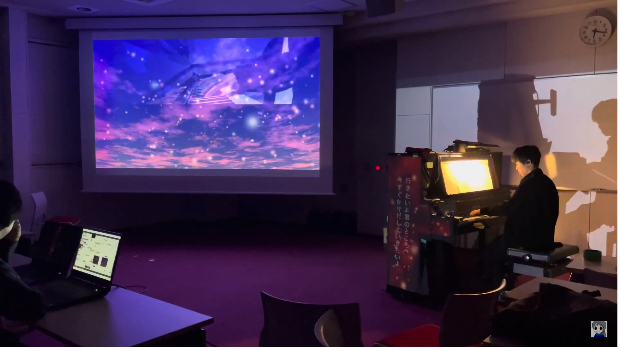
\includegraphics[width=\linewidth]{fig/fig5-planet-play}
    \caption{作品発表の様子}
    \label{fig:planet}
\end{figure}

\section{演奏者の魅力を引き出す演出表現}
3つ目の作品としてYOASOBIの「ラブレター」\cite{loveletter}における演出表現を行った．本作品では，トランペットとエレキギターの生演奏に合わせて部屋の壁一面を投影として，演出表現を行った．今回は，音楽が大好きな演奏者2人の気持ちを表現するような演出を施し，最後には両端に演奏者が大きく映し出されるようになっている．また，今回は生成AIを使用することで，より幅広く細かな表現を施すことができた．今後はより演奏者の動きや演奏に合わせた演出や，生演奏であることにこだわった見せ方をしたいと考えている．

\section{作品制作}
本研究では，身近な素材と技術を用いた作品制作を通して，空間における音楽映像体験を提供することを目的とした．今後はより空間全体を意識し，観客の視線誘導や演奏の自由度や，演奏者の動きを考慮した作品制作を行っていきたいと考える．

\vspace{12pt}
\small